\documentclass{report}

\usepackage{mathtools, amssymb}
\usepackage{caption}
\usepackage[utf8]{inputenc}
\usepackage{subcaption}
\usepackage{graphicx}

\graphicspath{ {images/} }

\DeclarePairedDelimiter{\abs}{\lvert}{\rvert}
\DeclarePairedDelimiter{\norm}{\lVert}{\rVert}

\title{%
 Visual Odometry for Navigating in GPS Denied Environments\\[1in]
  \large Final Report}

\date {August 2016}
\author{Alex Kreimer \\[1in] Department of Computer Science }

\begin{document}

\makeatletter
\begin{titlepage}
  \begin{center}
    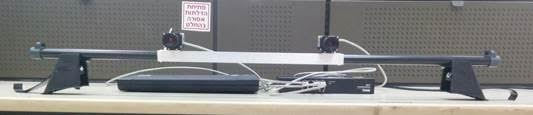
\includegraphics[width=0.7\linewidth]{title_cams}\\[4ex]
    {\huge \bfseries  \@title }\\[4ex] 
    {\LARGE  \@author}\\[50ex] 
  \end{center}
\end{titlepage}
\makeatother
\thispagestyle{empty}
\newpage

\begin{abstract}
  In this work we revisit the problem of visual odometry. Visual
  odometry is the process of estimating the motion of the camera by
  examining the changes that the motion induces on the images made by
  it. This work consists of two parts. In the first part we propose a
  novel visual odometry algorithm.  In the second part we describe a
  new data set.

  The algorithm we propose exploits a scene structure typical for that
  seen by a moving car and is suitable for use in either the stereo or
  the monocular setting.  We recover the rotation and the translation
  separately, thus dealing with two separate, smaller problems. The
  rotation is estimated by means of the infinite homography. The
  rotation estimation algorithm operates on distant image points using
  the 3-D to partition them into the distant and the near-by ones. We
  start with an initial estimate and then refine it using an iterative
  procedure. After the rotation is compensated for, the translation is
  found by means of the 1-point algorithm in the stereo setting and
  epipole computation for pure translational motion in the monocular
  setting.

  We also created a new dataset that contains stereo video tracks
  synchronized with the DGPS locations of the vehicle.  The dataset is
  suitable for future visual odometry experiments and is interesting
  because it has some challenging sequences (e.g. significant scene
  occlusions by a moving vehicle , fast camera motion, rural scenery,
  dusky sequences).
\end{abstract}

\tableofcontents{}

\chapter{Introduction}

Visual odometry refers to the problem of recovering camera motion
based on the images taken by it. This problem naturally occurs in
robotics, wearable computing, augmented reality and automotive.

Wheel odometry, recovers the motion of the vehicle by examining and
integrating the wheel turns over time.  In a similar manner, visual
odometry operates by estimating relative motion of the camera between
subsequent images by observing changes in them. Later, these estimates
are combined into a single trajectory. Just as in wheel odometry,
visual odometry is subject to error accumulation over time. Contrary
to wheel odometry, visual odometry is not affected by wheel slip in a
rough terrain. Visual odometry is able to produce motion estimates
with errors that are lower than those of the wheel odometry. Another
advantage of visual odometry is that cameras are low cost and low
weight sensors.  All these make visual odometry a viable supplement to
other motion recover methods such as global positioning systems (GPS)
and inertial measurement units (IMUs).

Visual odometry becomes a harder problem as the amount of detail in
the images diminishes. The images should have sufficient overlap and
the scene needs to be illuminated.  In the stereo setup, the scene
must be static or the images taken at the same time. Also, the video
processing incurs a computational burden.

Visual odometry is an active fields of research with a large amount of
published work.  We review only the most pertinent works.
~\cite{Scaramuzza2011} provides a more complete survey.

Similar to~\cite{Persson2015} we partition visual odometry algorithms
by four traits:
\begin{enumerate}
\item Feature-based vs direct
\item Global vs local
\item Filter based vs bundle adjustment based
\item Monocular vs stereo
\end{enumerate}

Visual odometry algorithms use large number of corner detectors (e.g.,
Moravec~\cite{Moravec1980}, Harris~\cite{Harris1987},
Shi-Tomasi~\cite{Shi1994}, Fast~\cite{Rosten2006}) and blob detectors
(e.g., SIFT~\cite{Lowe2004}, SURF~\cite{Bay2006}). Corners are faster
to compute and usually are better localized, while blobs are more
robust to scale change. The choice of a specific feature point depends
mainly on the images at hand.  Motion estimation results for different
feature points are presented in~\cite{Govender2009}. In this work we
choose Harris~\cite{Harris1987} corners, but this choice is not
crucial. We view the feature point choice as a parameter, which needs
to be determined from the data (e.g., by cross-validation).

The features are either tracked~\cite{Hedborg2009} or
matched~\cite{Geiger2011} (i.e., freshly detected in each new frame)
between subsequent images. While the early works chose to track
features, most of the current works detect and match them. The output
of this stage are pairs of the image features, which are the
projections of the same 3-D point.

Matched features are used as an input for a motion estimation
procedure.  Whether the features are specified in 2-D or 3-D, the
estimation procedures, may be classified into 3-D-to-3-D
~\cite{Milella2006}, 3-D-to-2-D ~\cite{Geiger2011} and 2-D-to-2-D
~\cite{Nister2004}. Most of the early works were of the 3-D-to-3-D
type.  More recent works~\cite{Nister2004} claim that this approach is
inferior to the latter two. Popular techniques that participate in
most algorithms in some way are essential matrix estimation and
(possibly) its subsequent decomposition~\cite{Nister2004}, perspective
3-point algorithm~\cite{Kneip1991}, and re-projection error
minimization~\cite{Geiger2011}.

Global methods~\cite{Klein2007},~\cite{Newcombe2011} keep the map of
the environment and make sure that motion estimates are globally
consistent with this map, while local methods do not.  Some local
methods~\cite{Badino2013} also keep track of a (local) map, but the
underlying philosophy is different: global vs local.  Global methods
usually more accurate since they make use of a vast amount of
information (which, of course, comes at a computational price).  Note
that accuracy does not imply robustness, since outliers that made
their way into the map may greatly skew subsequent pose estimates.

Methods that explicitly model system state uncertainty tend to use
filtering mathematical machinery,
e.g.,~\cite{Konolige2010},~\cite{Olson2003},~\cite{Kaess2008}.
Another alternative to maintain map/pose estimate consistency is to
use the bundle adjustment approach~\cite{Triggs2000}. Monocular
systems~\cite{Song} make use of a single camera, while stereo
systems~\cite{Geiger2011} rely on a calibrated stereo rig. In the
monocular setup the translation of the camera may only be estimated up
to scale, while in stereo all six motion parameters may be
recovered. An additional advantage of the stereo setup is that more
information is available at each step, which may be one of the reasons
why stereo algorithms perform better.

\chapter{The Infinite Visual Odometry Algorithm}

\subsection{Summary of Our Work}
In this work we present a novel algorithm for camera motion
estimation.  The novelty of the algorithm is in camera rotation
estimation procedure.  We rely on the fact that for scene points that
are infinitely far from the camera, the motion of the projected
(image) points may be described by an homography (the infinite
homography). For distant points this assumption is nearly true.  Our
algorithm starts by partitioning the scene points into two sets:
distant and near-by. Then, camera rotation is estimated from the
distant points and, subsequently, the translation is recovered from
the near-by points.

With respect to the classification of the visual odometry methods
given in the introduction, our work is local, feature based, stereo
odometry.  We do not use bundle adjustment, however the results of our
algorithm may be subsequently improved with some form of bundle
adjustment.

The outline of the our method:
\begin{enumerate}
\item Feature detection.  We use Harris~\cite{Harris1987} corners.
\item Feature matching. The matching is done both across the stereo
  pair images as well as previous vs.\ current pair.  We enforce
  epipolar constraint, chierality and use circle heuristics similar
  to~\cite{Geiger2011} to reject outliers.
\item Partition the scene points into two sets: distant and near-by.
\item Estimate the rotation of the camera from the distant points.
\item Estimate the translation of the camera from the near-by points.
\end{enumerate}

We choose the work~\cite{Geiger2011} as our baseline (our
implementation of their work).  The results in the
Section~\ref{sec:results} show that on the KITTI dataset our rotation
estimation method outperforms the baseline.

We also build a dataset that contains a number of sequences that may
be used to benchmark visual odometry algorithms.  We install
synchronized stereo pair along a (D)GPS receiver on a car that travels
in an urban as well as rural areas.  Our goal is to cover some
challenging conditions that happen in day-to-day driving, e.g., field
of view occlusions, poor lighting conditions and low texture areas.

Note, that budget constraints led us to a simplified system that is
capable of producing 3DOF data (i.e., location only) being unable to
track vehicle orientation.

\section{Preliminaries and Notation}

\subsection{Image Point Mapping Related to Camera Motion}

Suppose the camera matrices are those of a calibrated stereo rig
$\mathrm{P}$ and $\mathrm{P}'$ with the world origin at the first
camera

\begin{equation}
\mathrm{P = K[I\ |\ 0],\quad P'=K'[R\ |\ \mathbf{t}]}.
\end{equation}

Consider the projections of a 3D point $\mathbf{X}=(X,Y,Z,1)^T$ into the image
planes of both views:

\begin{equation}
\mathrm{\mathbf{x} = P\mathbf{X}, \quad \mathbf{x}' = P'\mathbf{X}}.
\end{equation}

If the image point is normalized as $\mathbf{x} = (x,y,1)^T$ then
\[
\mathbf{x}Z = \mathrm{P\mathbf{X} = K[I\ |\ 0]\mathbf{X} = K}(X,Y,Z)^T.
\]

It follows that $(X,Y,Z)^T = \mathrm{K^{-1}}\mathbf{x}Z$, and:
\begin{align}
  \mathbf{x}' &= \mathrm{K'[R\ |\ \mathbf{t}]}(X,Y,Z,1)^T \\
  &= \mathrm{K'R}(X,Y,Z)^T + \mathrm{K'\mathbf{t}}\\
  &= \mathrm{K'RK^{-1}}\mathbf{x}Z + \mathrm{K'\mathbf{t}}.
\end{align}

We divide both sides by $Z$ to obtain the mapping of an image point $\mathbf{x}$ to image point $\mathbf{x}'$

\begin{equation}
  \label{eq:general_point_motion}
  \mathbf{x}' = \mathrm{K'RK^{-1}}\mathbf{x} + \mathrm{K'}\mathbf{t}/Z = \mathrm{H_\infty}\mathbf{x}+ \mathrm{K'}\mathbf{t}/Z = \mathrm{H_\infty}\mathbf{x} + \mathbf{e'}/Z.
\end{equation}

$\mathrm{H_\infty}$ is the infinite homography that transfers the
points at infinity to the points at infinity.  If $\mathrm{R = I}$
(e.g., pure translation) the point $\mathbf{x}$ will undergo a motion
along a corresponding epipolar line:
\begin{equation}
\mathbf{x}' = \mathbf{x}+ \mathrm{K'}\mathbf{t}/Z = \mathbf{x}+\mathbf{e}'/Z.
\end{equation}

If $\mathbf{t} = \mathbf{0}$ the motion of the point may be represented by a homology:
\begin{equation}
\mathbf{x}' = \mathrm{H_\infty}\mathbf{x}.
\end{equation}

\begin{figure}[h]
  \centering
  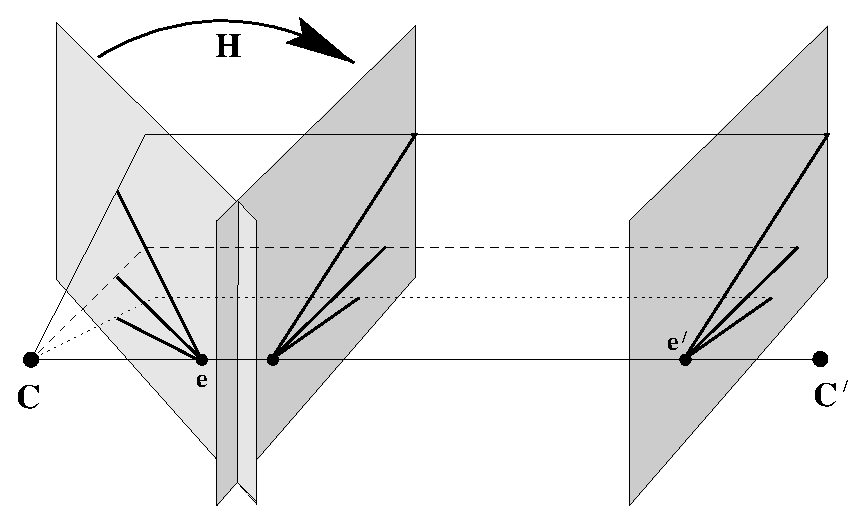
\includegraphics[scale=.5]{fig89}
  \caption{(Adapted from~\cite{Hartley2004}) The effect of the camera motion on
    the image points may be viewed as a two-step process: mapping by a
    homography $\mathrm{H_\infty}$ followed by a motion along the corresponding
    epipolar lines.}
  \label{fig:two_step_motion}
\end{figure}

In a general case the mapping of an image point $\mathbf{x}$ into
$\mathbf{x}'$ may be viewed as a two step process: transformation by a
homology (a specialization of homography which has two equal
eigenvalues) $\mathrm{H_\infty}$ which simulates a pure rotational
motion of the camera followed by an offset along the epipolar line
which simulates a pure translational motion of the camera, see Figure~\ref{fig:two_step_motion}.

\section{Motion Estimation}\label{sec:moest}

Our strategy to attack the problem is to separate it into two smaller
sub-problems: rotation estimation and translation estimation. The
algorithm relies on the ability to partition the scene points into two
sets: the distant and the near-by ones.  The distant points are used
for rotation estimation while the near-by ones take part in the
translation estimation.

First, the stereo algorithm is presented, followed by the monocular
one.  The main difference is in the translation estimation part. While
it is possible to implement a stereo-like algorithm in the monocular
setting as well, it suffers from the scale drift.  Thus, we propose a
different technique.


\subsection{Stereo}\label{sec:stereo_moest}
\paragraph{Partitioning the points} To partition the points in the
stereo case we hard-threshold their $Z$-coordinates (the threshold is
a parameter of the algorithm).  The depth of the points was computed
by a stereo triangulation.

\paragraph{Rotation Estimation:}\label{sec:rotation_estimation}
We use distant points to estimate rotation $\mathrm{R}$ (i.e., near-by
points do not take part in rotation estimation). As Eq.
(\ref{eq:general_point_motion}) states:

\begin{equation}
  \mathbf{x}' = \mathrm{KRK^{-1}}\mathbf{x} + \mathrm{K}\mathbf{t}/Z.
\end{equation}

The total motion of the feature point in the image plane may be viewed
as a two-step process (the order is not important): transformation by
homography $\mathrm{H_\infty} = \mathrm{KRK^{-1}}$ followed by
displacement along the line defined by the epipole $e'$ and the point
$\mathrm{H_\infty}\mathbf{x}$.  The magnitude of the displacement
along the epipolar line depends on the the camera translation and the
inverse depth of the point, see Figure~\ref{fig:feature_motion}.

\begin{figure}[h]
  \centering
  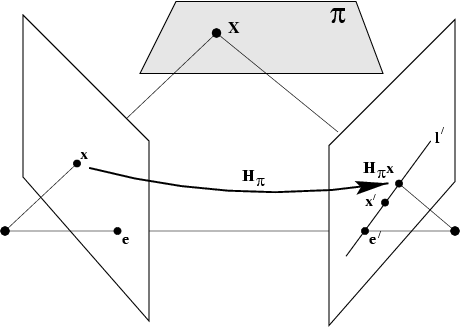
\includegraphics[scale=.5]{fig85_adapted}
  \caption{(Adapted from~\cite{Hartley2004}) The homography $H_\pi$ transfers the point onto a corresponding epipolar line.  The displacement along the epipolar line depends on the inverse depth of the point and the camera translation magnitude.}
  \label{fig:feature_motion}
\end{figure}                                                             %

Our estimation algorithm consists of initialization and non-linear
refinement.
\paragraph{Initialization:} to compute the initial estimate of the rotation
parameters we assume that for the distant points (s.t., $\norm{\mathbf{t}}/Z \ll \norm{\mathrm{H_\infty}\mathbf{x}}$):

\begin{equation}\label{eq:homography_transfer}
  \mathbf{x}' \approx \mathrm{KRK^{-1}}\mathbf{x}.
\end{equation}

This assumption is justified by the fact that for the distant points
the displacement along the epipolar line is small. We multiply
both sides of Eq. (\ref{eq:homography_transfer}) by $\mathrm{K^{-1}}$
and denote $\mathbf{u'} = \mathrm{K^{-1}}\mathbf{x}$ and
$\mathbf{u} = \mathrm{K^{-1}}\mathbf{x}$:

\begin{equation}
  \mathbf{u'} = \mathrm{K^{-1}}\mathbf{x}' \approx \mathrm{RK^{-1}}\mathbf{x} = \mathrm{R}\mathbf{u}.
\end{equation}

Since $\mathbf{u}$ and $\mathbf{u}'$ are projective quantities, only
their directions are of importance, we normalize them to unit length
and denote normalized quantities by $\mathbf{\tilde{u}}$ and
$\mathbf{\tilde{u}}'$ respectively. We choose a sample of $n$ points
($n=3$) and stack them as columns of matrices $\mathrm{\tilde{U}}$ and
$\mathrm{\tilde{U}'}$ respectively.  We search for $\mathrm{R}$ that
solves the following minimization problem:

\begin{equation}\label{eq:absolute_orientation}
\underset{\mathrm{R}}{\text{argmin}}\ \norm{\mathrm{\tilde{U}'-R\tilde{U}}}_2.
\end{equation}

Eq. (\ref{eq:absolute_orientation}) is known as the absolute
orientation problem (see e.g.,~\cite{Horn1987}) and its solution
provides an initial estimate for the subsequent non-linear
optimization problem.

\paragraph{Refinement:} The idea of the refinement is this: the
residual vector $\mathrm{H}_\infty\mathbf{x} - \mathbf{x}'$ may be
viewed as a sum of a vector orthogonal to the epipolar line and the
vector parallel to it.  We search for the camera rotation that ignores
the parallel component (we view it as a ``legal'' bias) while trying
to minimize the orthogonal one.  We define the point residual as the
orthogonal distance to the corresponding epipolar line and minimize
the sum of squared residuals for all points.  We do so, because, as
Eq. (\ref{eq:general_point_motion}) suggests, after we compensate for
a rotation, the point is still allowed to move along the epipolar
line.

Consider the objective:

\begin{equation}\label{eq:refinement_objective}
  \begin{split}
    \mathrm{R(v,\theta)} = \underset{v,\ \theta}{\mathrm{argmin}}
    \sum_{i=1}^N{r_i}^2\quad \text{s.t.}\quad r_i&=n_i\cdot (\mathbf{x}_i'-H_\infty(v,\theta)\mathbf{x}_i) \\
    \text{where}\ n_i &= (\mathrm{F}\mathbf{x}_i)_\perp
  \end{split}
\end{equation}
$\mathrm{H_\infty}(v,\theta) = \mathrm{KR(v,\theta)K^{-1}}$ is the
homography that transforms the image points in Eq.
(\ref{eq:general_point_motion}). It depends on a known camera
intrinsic matrices $\mathrm{K}$ and a rotation matrix $\mathrm{R}$.
We choose to parameterize the rotation by an angle $\theta$ and an
axis $v$.  $\mathrm{F}$ denotes the fundamental matrix that
corresponds to two subsequent stereo rig poses and is computed
elsewhere. $\mathrm{F}\mathbf{x}_i$ denotes the epipolar line that
corresponds to $\mathbf{x}_i$ in the second image and
$(\mathrm{F}\mathbf{x}_i)_\perp$ is the normal to this line.
We solve the minimization problem
(\ref{eq:refinement_objective}) by means of the Levenberg-Marquardt
optimization algorithm.

To make the estimation robust we wrap the initialization procedure
into the RANSAC iterations.  We choose the strongest consensus
estimate and its support set as an input for the solution of the
Eq. (\ref{eq:refinement_objective}).

\paragraph{Translation Estimation (1-point
  algorithm)}\label{sec:stereo_trans} To estimate
the translation we use only the near-by points.  First, we triangulate
these points in the previous stereo pair to obtain their 3-D
locations, and then iteratively minimize the sum of reprojection
errors into the current frame.

The reprojection of point $\mathbf{X}=(X,Y,Z,1)^T$ into the current
left image is given by:
\begin{equation}
  \pi^{(l)}(\mathbf{X};\mathbf{t}) =  K\Bigl[ \mathrm{R}\ |\ \mathbf{t} \Bigr]\mathbf{X}.
\end{equation}
and the reprojection of the same point into the current right image
($b$ is the baseline of the stereo-rig) is given by:
\begin{equation}
  \pi^{(r)}(\mathbf{X};\mathbf{t}) =  K\Bigl[ \mathrm{R}\ |\ \mathbf{t} \Bigr](\mathbf{X} - (b,0,0,0)^T),
\end{equation}

We use the Levenberg-Marquardt algorithm to iteratively minimize the
sum of squared reprojection errors (starting from
$\mathbf{t}=\mathbf{0}$):
\begin{equation}
\norm{\mathbf{x'} - \pi^{(l)}(\mathbf{X};\mathbf{t})}^2 + \norm{\mathbf{x'} - \pi^{(r)}(\mathbf{X};\mathbf{t})}^2.
\end{equation}

There are three unknown parameters, since
$\mathbf{t} = (t_x,t_y,t_z)^T$, thus a single 3-D point provides
enough constraints to determine $\mathbf{t}$.

\section{Experimental Results}\label{sec:results}

\subsection{The Choice of Features}
We chose to evaluate our algorithm on the KITTI
dataset~\cite{Geiger2012}, which is a de-facto standard for the
visual odometry research works.

\paragraph{Feature Detector/Descriptor:} We use Harris
~\cite{Harris1988} corner detector. It is fast, well localized and
(most important) Harris corners are abundant in urban scenes we work
with. We detect corners in each new image and then match them to
obtain putative matches.  We tune sensitivity threshold of the
detector in such a way, that we are left with about five hundred
putative matches after matching and pruning.  We extract a square
patch of $7\times 7$ pixels centered at the corner point and use this
vector as feature descriptor.

We would like to point out that our method may be used with any
feature detector that would allow to match features across images. The
choice of feature detector should be viewed as a parameter to the
algorithm and mainly depends on the images at test.

\paragraph{Feature Matching:} We use sum-of-square differences (SSD)
of feature descriptors as a metric function when matching
features. For each feature we choose a single best match w.r.t. the
metric function in the other image. We employ a number of heuristics
to prune outliers:
\begin{itemize}
\item Reciprocity: features $a$ and $b$ match only if $a$ matches $b$
  and $b$ matches $a$
\item Epipolar constraint: we work with calibrated stereo pair.  When
  we match features across images of stereo pair, the search is
  one-dimensional, i.e., along the horizontal epipolar line.  This
  heuristic is not used when matching features across subsequent
  frames.
\item Chierality (visibility): also used when matching features across
  stereo pair images.  We triangulate the features to obtain the 3-D
  point and keep the match only if the 3-D point is visible in both
  cameras.
\item Circular match: similar to ~\cite{Geiger2011} we keep only those
  matches that form a circle.
\end{itemize}

\subsection{Experimental Results}

The Tables \ref{table:rot_err} and \ref{table:trans_err} present the
results of the experiments for the KITTI dataset. The columns denote
the number of the sequence.  The rows denote the algorithm: SS is the
baseline, HX is the stereo version of the algorithm.  The numbers are
the mean error for the corresponding sequence with the last column is
the mean error for the dataset. The error computation method is
described in~\cite{Geiger2012}.

\paragraph{Stereo} In this set of experiments we ran our algorithm in
its stereo mode as described in the Section \ref{sec:stereo_moest}.
Table \ref{table:rot_err} and \ref{table:trans_err} present the
rotation and the translation errors respectively in the row HX. The
columns marked bold are those that our algorithm outperforms the
baseline (on 9 of 11 sequences). The results show that our algorithm improves the
rotation results over the benchmark algorithm and successfully
competes with it in the translation estimation.

\paragraph{Mono} In an additional set of experiments we ran our
algorithm in a monocular mode. Monocular motion estimation lacks a
scale parameter. In order to compare the results we set the
scale of the translation to be that of the stereo algorithm.  Feature
point selection/partition was done without using any stereo
information and the motion estimation was done as explained in the
Section~\ref{sec:mono_moest}.

\section{Conclusions and Discussion}
This paper presents a novel visual odometry algorithm.  The novelty of
the algorithm is in its rotation estimation method.  The rotation is
estimated by means of the infinite homography.  The algorithm may be
used both in the stereo and in the monocular setting.

The strengths of the presented algorithm are in its ability to split
the motion estimation problem into two smaller problems and to operate
directly on the image points instead of on the computed 3-D
quantities.  Splitting the problem helps because each sub-problem is
easier to solve.  The ability to partition the points into the distant
and the near-by ones is what allows us to separate the rotation and
the translation estimation.  

The stereo version of the algorithm shows better performance, but the
monocular version has the advantage of being a more practical one.
Indeed the authors in~\cite{Geiger2012} report that they re-calibrate
the cameras before each drive, which is hardly possible in real world
installations.

\begin{table}
  \centering
  \caption{Rotation errors for the KITTI sequences [deg/m]}
  \label{table:rot_err}
  \smallskip\noindent
  \resizebox{\linewidth}{!}{%
    \begin{tabular}{|c|c|c|c|c|c|c|c|c|c|c|c|c|}
\hline
 & 00 & 01 & 02 & 03 & 04 & 05 & 06 & 07 & 08 & 09 & 10 & mean \\
\hline
SS & 3.95e-04 & 1.98e-04 & 4.11e-04 & 1.07e-03 & 8.03e-04 & 3.49e-04 & 4.72e-04 & 2.96e-04 & 3.69e-04 & 3.44e-04 & 4.82e-04 & 4.71e-04 \\
\hline
HX & \textbf{2.70e-04} & \textbf{1.75e-04} & \textbf{4.10e-04} & \textbf{6.51e-04} & \textbf{6.04e-04} & 3.95e-04 & \textbf{3.77e-04} & \textbf{2.37e-04} & \textbf{3.23e-04} & \textbf{3.22e-04} & 5.66e-04 & \textbf{3.93e-04} \\
\hline
\end{tabular}

  }
\end{table}

\begin{table}
  \centering
  \caption{Translation errors for the KITTI sequences \% }
  \label{table:trans_err}
  \smallskip\noindent
  \resizebox{\linewidth}{!}{%
    \centering
\begin{tabular}{|c|c|c|c|c|c|c|c|c|c|c|c|c|}
\hline
 & 00 & 01 & 02 & 03 & 04 & 05 & 06 & 07 & 08 & 09 & 10 & mean \\
\hline
SS & 4.40e+00 & 9.25e+00 & 4.03e+00 & 1.22e+01 & 5.06e+00 & 2.80e+00 & 4.37e+00 & 2.21e+00 & 4.12e+00 & 5.25e+00 & 5.60e+00 & 5.39e+00 \\
\hline
HX & 3.07e+00 & 1.08e+01 & 3.80e+00 & 7.94e+00 & 3.82e+00 & 4.06e+00 & 3.99e+00 & 1.67e+00 & 3.28e+00 & 3.77e+00 & 5.65e+00 & 4.72e+00 \\
\hline
\end{tabular}

%%% Local Variables:
%%% mode: latex
%%% TeX-master: t
%%% End:

  }
\end{table}

\chapter{The Dataset}
\section{Data Acquisition}

\subsection{Overview}
Our system consist of a synchronized stereo pair and a GPS receiver synced to the cameras.  During the recording process GPS device produces a clock signal of 10 Hz that triggers the cameras.  The data is written to PC that is connected to both the cameras and the GPS.

\subsection{Physical Setup}
\paragraph{The cameras} We use a pair of 3Mp Ethernet IDS-Imaging
cameras UI-5240SE.  Hardware synchronization is made by external
vendor and uses built-in camera-flash sync option.  It allows us to
capture images at about the same time (empirically measured time delta
is around single digit in ms).  Low skew is essential for the stereo
algorithms.  If the time delta is significant, static scene assumption
breaks rendering stereo pair useless.  The sync quality depends on the
vehicle velocity as well. We built a system suitable for regular
driver usecase.

Another rig parameter is the baseline (i.e., distance between the
cameras).  We tend to be close to KITTI setup in this sense.

Another area of concern is the amount of data such stereo rig
produces.  We shoot at 10 FPS which makes it about 3*2*10 = 60 Mb/s.
On top of this the system needs to work at a moving vehicle, which
rules out non-SSD hard drives.

The cameras are fixed focus and auto-exposed.  Auto exposure is
critical for outside scenes, especially on a high-contrast sunny day.

\paragraph{The GPS} Consumer grade GPS measurements expected accuracy
are about 3-5 m. This is not the same order of magnitude as state of
the art visual odometry algorithms.  On the other hand VO suffers from
dead-reckoning (e.g. error accumulation) while GPS error is absolute
and constant.  In our work we use Differential GPS correction to
improve the expected accuracy of the GPS measurements.  An enabler for
such correction is the raw GPS data (e.g., pseudoranges, satellites
availability, signal strengths, etc.)

After evaluation we chose UBLOX Neo-7P as an inexpensive device that
suites our needs.  It is able to both produce the raw measurement data
and to trigger the cameras.  The schematic drawing of the system is
presented in Figure 2.  UBLOX is connected to the PC through USB and
to the cameras by means of electric wire.  It triggers the cameras at
10 Hz and produces GPS measurements synced to the images at 1 Hz.

\begin{figure}[h]
\centering
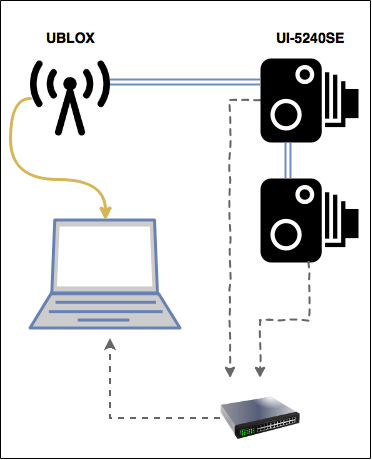
\includegraphics[width=.5\textwidth]{schema}
\caption{Schematic depiction of the system}
\end{figure}

\paragraph{The Software} Our system uses a number of software packages
for data recording and post-processing.

We use IDS Imaging software suite to record the image sequences.  The
sequences recorded as video files at 10 FPS.  This software allows us
to track the quality of the recording, e.g., if there are lost frames,
which improves the quality of the data.

We use goGPS open source positioning software to record GPS data.  Our
setup is a bit unusual and thus it is rather hard to find out of the
box software that is capable to synchronize the GPS and the cameras.
We use MATLAB version of the software. We modified out of the box
version to communicate with UBLOX device.  The modification we made
allows us to tell UBLOX to issue a sync pulse to the cameras, which is
essential to us.

\paragraph{The experiment day} We install the camera rig and the GPS
antenna on the roof our lab vehicle.  The whole system is powered by
the vehicle.  At the beginning of each day we re-calibrate the stereo
rig to make sure the calibration data is correct.

We usually record a few minute length video tracks along with the GPS
tracks.  The data is stored on the PC for further post-processing.

\section{Post-processing}
\subsection{Image sequences}
At this stage we: Compute the calibration data from the calibration
board images Split video files to produce image sequences Rectify
image sequences.

We use OpenCV calibration toolbox for these tasks.  We bundle this
code with the project.

\subsection{GPS Data} First we perform the DGPS correction.  The idea
of this correction is simple: use a known-location base-station to
correct the vehicle position measurement.  While the idea is simple,
there are a lot of technicalities (e.g., which satellites should be
taken into consideration and what the weight of their pseudo-ranges
should be in the computation).  This may be done in real-time or
offline.  Budget constraint did not allow us to obtain equipment that
is capable of real-time correction, thus we do it offline.

We obtain Israel Mapping Center data for the experiment day.  There is
a base-station on Technion campus.  This is important, since the
reliability of the correction decays as the distance to the
base-station.  It is common wisdom, that the correction is reliable
for <10 Km baselines (e.g. the distance between the vehicle and the
base-station).  We tried to respect this rule when doing our
experiments.

All the correction heavy-lifting is done by the RTKLib software
package.  RTKLib correction outputs measurement timestamp, WGS84
location and its covariance, along with some additional data.  The
example is in the figure below:

\subsection{Missing GPS Data}

RTKlib may disregard a certain measurement because of its quality
(e.g., if RTKLib is sure that the measurement is wrong).  In this case
the file will have a gap in time stamps.  We provide missing data
information as a part of the final dataset.

\section{VO results evaluation}

There is a number of ways to compare VO and DGPS data, but all of the assume that both the GPS track and the VO track are in the same reference frame, which is not the case with our data.

While GPS locations are provided in Earth Centered WGS84 coordinate frame,  Visual Odometry data is usually computed relative to the initial position/orientation of the camera.  Thus, before the results may be compared to the ground-truth they need to be represented in the same coordinate frame.

To represent both tracks in the same reference frame we use the following procedure:
Subtract the location of first GPS measurement from all GPS measurements.  This effectively brings the origin of the GPS measurements into the location of the first camera instead of being earth centered.
Rotate the VO track to coincide with the GPS data.

To compute the rotation we propose the following procedure: let A be the matrix with VO measurements stacked as its rows, and let Bbe the matrices with GPS measurements stacked as its rows.  We search for the rotation matrix R, s.t. 
argmin iRA(:,i)-B(:,i)2 
This optimization problem is called absolute orientation problem in the literature and has an SVD and quaternion based solutions (see e.g., [1] for reference).

\begin{table}[h!]                                                                     
\centering
\resizebox{\columnwidth}{!}{%
\begin{tabular}{|c|c|c|c|}                                                            
\hline    
 & Distance Travelled [m] & Total Number of Measurements & Number of Valid Measurements \\
\hline
02 & 349.042 & 104 & 104 \\
\hline
03 & 2369.983 & 152 & 152 \\
\hline
04 & 1507.547 & 145 & 145 \\
\hline
05 & 2551.071 & 227 & 227 \\
\hline
06 & 4696.472 & 369 & 368 \\
\hline
07 & 2565.551 & 357 & 289 \\
\hline
08 & 1886.901 & 235 & 235 \\
\hline
09 & 1887.352 & 241 & 241 \\
\hline
10 & 3022.444 & 269 & 269 \\
\hline
12 & 2466.176 & 379 & 326 \\
\hline
13 & 3521.839 & 262 & 212 \\                                                              
\hline                                                                                    
14 & 4856.919 & 437 & 361 \\                                                              
\hline                                                                                    
15 & 4137.280 & 332 & 332 \\                                                              
\hline                                                                                    
16 & 3190.590 & 343 & 328 \\                                                              
\hline                                                                                    
17 & 2032.794 & 321 & 320 \\                                                              
\hline                                                                                    
18 & 1190.792 & 166 & 165 \\                                                              
\hline                                                                                    
19 & 1432.072 & 216 & 214 \\                                                              
\hline                                                                                    
total & 43664.824 & 4555 & 4288 \\                                                        
\hline                                                                                    
\end{tabular}                                                                         }    
\caption{Dataset details}
\label{table:MyTableLabel}                                                            
\end{table} 

\begin{figure}
  \begin{minipage}[b]{.5\textwidth}
    \centering
    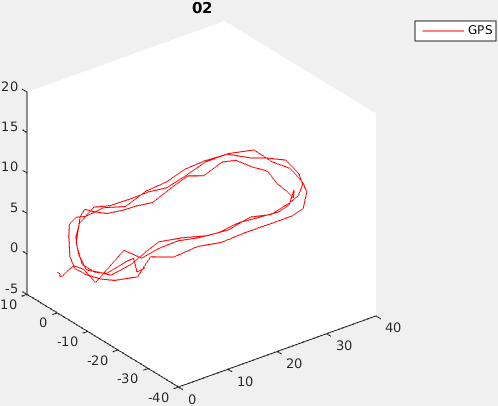
\includegraphics[width=.9\textwidth]{02_path}
  \end{minipage}%
  \begin{minipage}[b]{.5\textwidth}
    \centering
    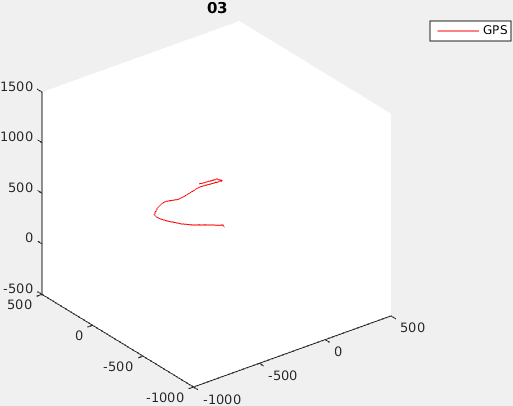
\includegraphics[width=.9\textwidth]{03_path}
  \end{minipage}
  \begin{minipage}[b]{.5\textwidth}
    \centering
    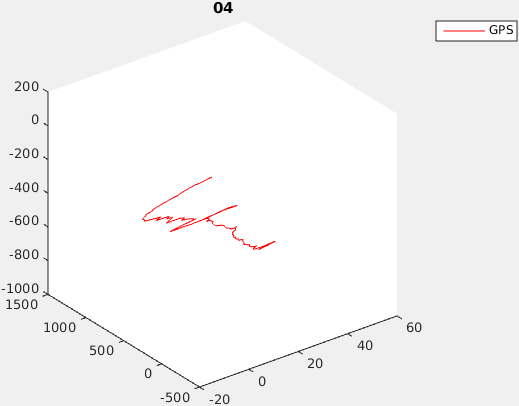
\includegraphics[width=.9\textwidth]{04_path}
  \end{minipage}%
  \begin{minipage}[b]{.5\textwidth}
    \centering
    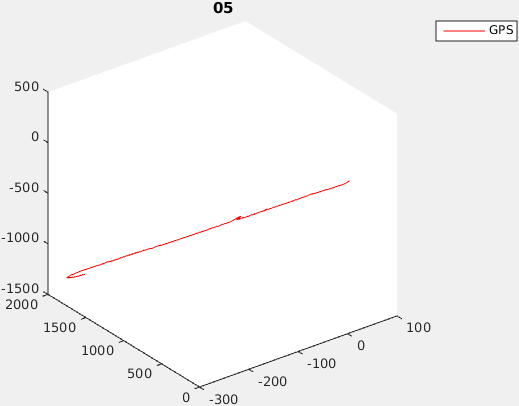
\includegraphics[width=.9\textwidth]{05_path}
  \end{minipage}
  \begin{minipage}[b]{.5\textwidth}
    \centering
    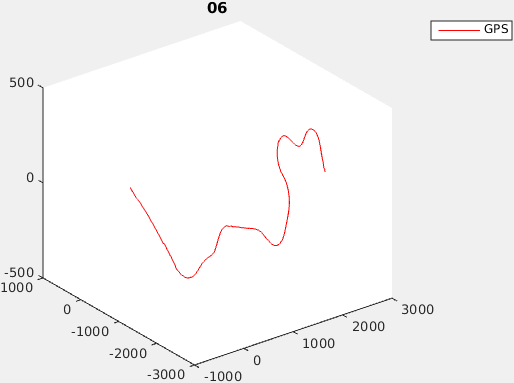
\includegraphics[width=.9\textwidth]{06_path}
  \end{minipage}%
  \begin{minipage}[b]{.5\textwidth}
    \centering
    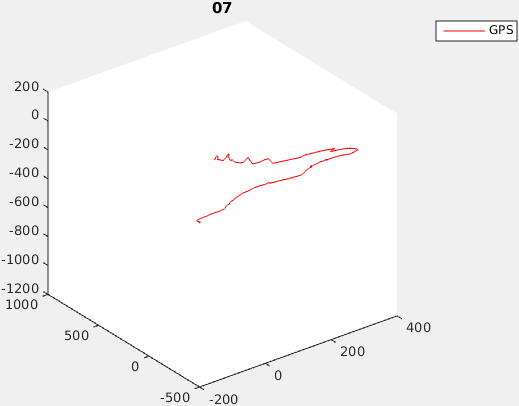
\includegraphics[width=.9\textwidth]{07_path}
  \end{minipage}

  \begin{minipage}[b]{.5\textwidth}
    \centering
    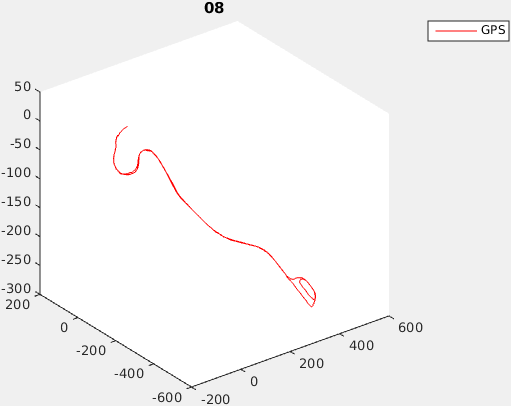
\includegraphics[width=.9\textwidth]{08_path}
  \end{minipage}%
  \begin{minipage}[b]{.5\textwidth}
    \centering
    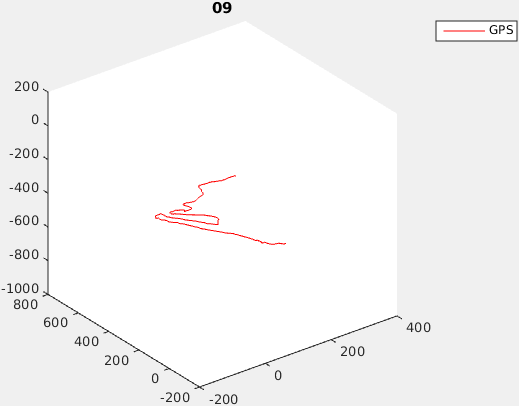
\includegraphics[width=.9\textwidth]{09_path}
  \end{minipage}
  \caption{Eight sequences, note the difference in axis scales}
\end{figure}

\begin{figure}
  \begin{minipage}[b]{.5\textwidth}
    \centering
    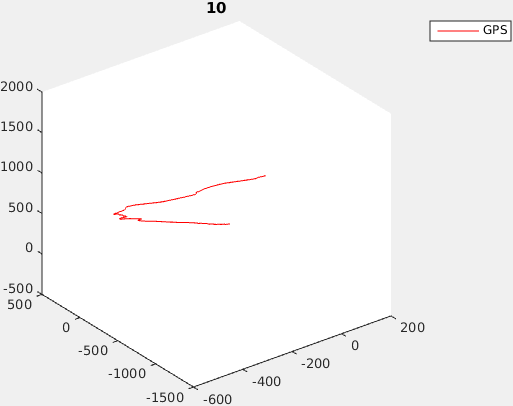
\includegraphics[width=.9\textwidth]{10_path}
  \end{minipage}%
  \begin{minipage}[b]{.5\textwidth}
    \centering
    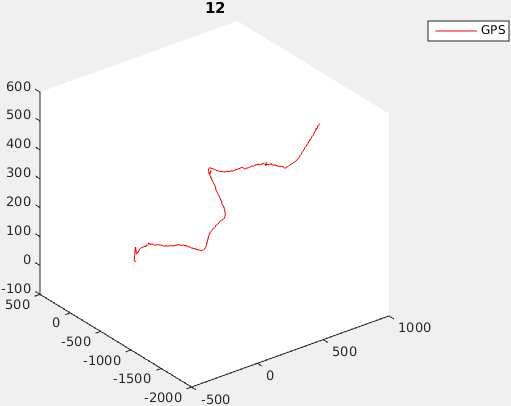
\includegraphics[width=.9\textwidth]{12_path}
  \end{minipage}
  \begin{minipage}[b]{.5\textwidth}
    \centering
    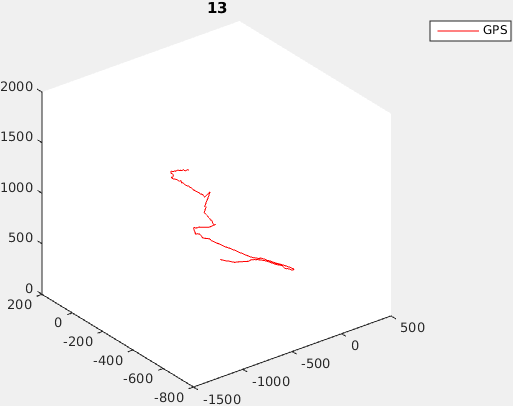
\includegraphics[width=.9\textwidth]{13_path}
  \end{minipage}%
  \begin{minipage}[b]{.5\textwidth}
    \centering
    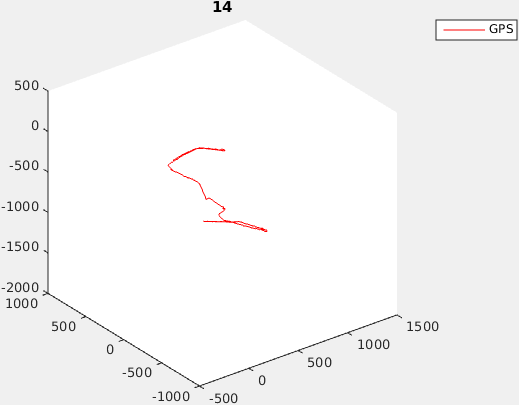
\includegraphics[width=.9\textwidth]{14_path}
  \end{minipage}
  \begin{minipage}[b]{.5\textwidth}
    \centering
    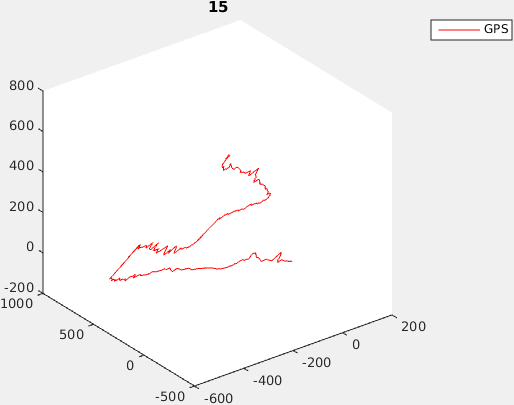
\includegraphics[width=.9\textwidth]{15_path}
  \end{minipage}%
  \begin{minipage}[b]{.5\textwidth}
    \centering
    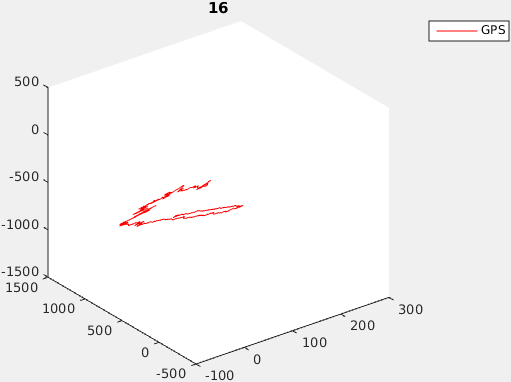
\includegraphics[width=.9\textwidth]{16_path}
  \end{minipage}
  \begin{minipage}[b]{.5\textwidth}
    \centering
    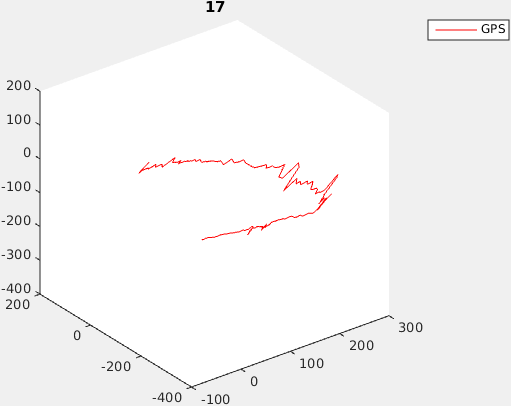
\includegraphics[width=.9\textwidth]{17_path}
  \end{minipage}%
  \begin{minipage}[b]{.5\textwidth}
    \centering
    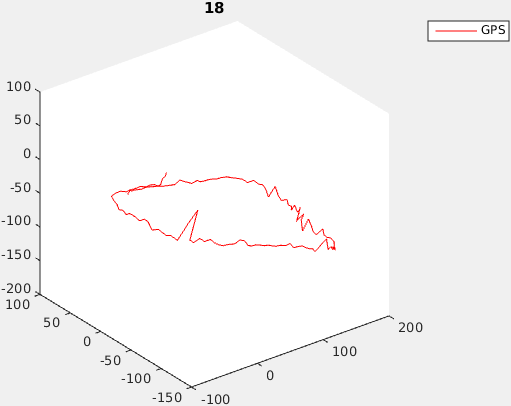
\includegraphics[width=.9\textwidth]{18_path}
  \end{minipage}

  \caption{Eight more sequences}
\end{figure}

\begin{figure}
  \begin{minipage}[b]{\textwidth}
    \centering
    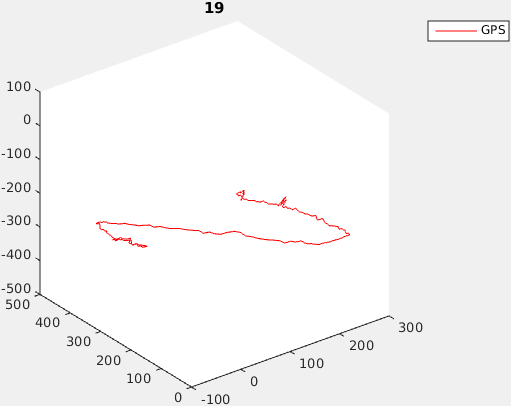
\includegraphics[width=.5\textwidth]{19_path}
  \end{minipage}%

  \caption{One more sequence}\label{fig:1}
\end{figure}

\clearpage
\bibliographystyle{plain}
\bibliography{egbib}
\end{document}

%%% Local Variables:
%%% mode: latex
%%% TeX-master: t
%%% End:
